%% main.tex — Anvil paper (thread: conformal-antenna-diffopt, version .4)
%% Framing-repair + citation-wiring pass by anvil:paper-revise from .3 against
%% the .3.litsearch critic sibling (#659 pre-submission novelty re-scan,
%% 2026-07-21). Fifteen verified references added and argued (Tidy3D autograd,
%% SSP/SSP2, PNGF, FDTDX JOSS, adjacent PEC-shape / integral-equation work),
%% the two mandatory scoping sentences landed (curved-metal driven-port claim;
%% matched-fidelity intractability comparison), and the #659 operator pass
%% reapplied (public repo URL; hughes2019forward / hammond2022meepadjoint /
%% oskooi2010meep / erentok2011topology wired into intro + related work + Sec. 5;
%% the two named-but-uncited disclaimer passages removed).
%% No number, method, result, figure, or title changed.
%% All numbers trace to artifacts committed on `main`:
%%   benchmarks/patch_antenna_conformal/conformal_results.toml  (headline design)
%%   benchmarks/fdtd_density_baseline/staircasing_results.json  (geometric-fidelity axis)
%%   benchmarks/fdtd_density_baseline/meep_runtime_scaling.json (compute axis)
%%   reference/meep/docker/                                      (FDTD-density baseline)
%% No fabricated or converged-FDTD-density number is asserted anywhere.

\documentclass{anvil-paper}

\title{Differentiable-by-Construction FEM for Freeform Open-Radiator Design:
A Curved Conformal Antenna Structured-Grid Inverse Design Cannot Reach}
\author{Robb Walters\\[2pt]
  {\small\itshape Independent Researcher}\\
  {\small\texttt{rjwalters@gmail.com}}}
\date{\today}

\begin{document}
\maketitle

\begin{abstract}
Differentiable electromagnetic (EM) simulators have made photonic inverse
design routine, but the dominant tools optimize a permittivity \emph{density}
field on a structured Yee/Cartesian grid, a representation that staircases
curved metal and is a poor fit for open radiators terminated by a perfectly
matched layer (PML). We present a tensor-compiled, differentiable-by-construction
3-D N\'ed\'elec H(curl) finite-element method (FEM) that exposes an exact,
single-factorization discrete \emph{shape} (moving-boundary / node-motion)
adjoint through the full open-radiator forward: a matched box-UPML tensor
material, lossy complex-$\varepsilon$ FR-4, and a lumped feed port assembled into
one complex-symmetric pencil $A(\omega)=K(\nu)-\omega^2 M(\varepsilon)+(j\omega/Z_s)S_p$.
Forward-mode ``Dual-twin'' element kernels give exact
$\partial K/\partial X,\ \partial M/\partial X,\ \partial b/\partial X$, so the
transpose adjoint reuses the single forward factorization
($n_{\text{fact}}=1$ per band frequency). We drive a high-DOF harmonic
mesh-morph parametrization (73 active boundary DOFs) to gradient-design a
\emph{freeform curved-metal conformal} radiator: the optimizer reaches a genuine
target-hit terminal that drives the entire design band below $-10$~dB return
loss (worst-of-band $-5.51 \to -12.06$~dB), with the band gradient FD-validated
at relative error $1.17\times10^{-10}$, enforced passivity $|S_{11}|\le1$, and a
non-inversion guard. We then \emph{measure} why a structured-grid density method
cannot reach the same design, on two independent axes committed to the
repository: geometric fidelity (rasterizing the curved conductor onto a Yee grid
leaves a perimeter error that does not vanish but plateaus at $\sim\!+14\%$;
$\sim\!1\,\mu$m boundary fidelity would need $\sim\!250$ cells/mm) and compute
(measured Meep scaling gives $\sim\!R^3$ cells and $\sim\!R^4$ wall-clock, so a
faithful discretization is computationally intractable for single-process,
single-node Meep~$1.34.0$ on a $61$~GB host --- a RAM wall by
$R\!\ge\!14$ on that $61$~GB box, $\sim\!10^{15}$ cells at the curve-faithful
resolution, with the higher-resolution and multi-node cost stated as a labeled
projection). We did not run a converged FDTD-density optimization; the
intractability is shown by measured scaling and projection, and such a run is
left as future work. We position the narrow, honestly-scoped novelty against
prior EM shape adjoints and the structured-grid density ecosystem.
\end{abstract}

\section{Introduction}
\label{sec:intro}

Inverse design has become the default workflow for nanophotonic components:
given a differentiable forward Maxwell solver, one back-propagates a
figure-of-merit to a large parameter vector and lets gradient descent discover
non-intuitive structures. The canonical ``killer'' demonstrations --- the
compact wavelength demultiplexer of Piggott et al.~\cite{piggott2015} and the
high-NA achromatic metalens of Chung and Miller~\cite{chung2020} --- are
guided-wave or periodic \emph{photonic} problems, and the workhorse tools
(\textsc{ceviche}~\cite{hughes2019forward}, Meep's adjoint
solver~\cite{hammond2022meepadjoint}, SPINS-B~\cite{su_spinsb},
FDTDX~\cite{fdtdx,mahlau2026fdtdx}, invrs-gym~\cite{invrsgym}) optimize a permittivity
\emph{density} field discretized on a structured Yee/Cartesian grid. This
representation is a superb fit for topology optimization of dielectric
photonics, but it has two structural mismatches with a large and practically
important class of RF/antenna problems: (i) it \emph{staircases} curved metal,
so a conformal radiator wrapped around a cylinder is only ever approximated at a
density-limited grid cost; and (ii) it optimizes ``where is there material''
rather than ``where is the metal boundary,'' which is the natural design
variable for a driven, PML-terminated \emph{open radiator}.

We take the differentiable-simulation lens to that underserved corner. The
substrate is a tensor-compiled, differentiable-by-construction 3-D N\'ed\'elec
H(curl) FEM on \emph{unstructured} tetrahedral meshes; the payload is a
moving-boundary shape-adjoint geometry class that treats the positions of the
conductor boundary nodes as the design variables and moves them --- the metal
boundary is represented exactly, at every step, on a body-fitted mesh. The
headline is a design result: end-to-end gradient design of a freeform
curved-metal conformal antenna that drives the entire design band below
$-10$~dB return loss. We then close the comparative loop the title asserts by
\emph{measuring}, on two committed axes, that a structured-grid density method
cannot practically reach the same design at the resolution the curved geometry
demands (Section~\ref{sec:eval}).

We are deliberately narrow about the novelty. Node-motion EM shape adjoints on
unstructured meshes already exist (Section~\ref{sec:related}); this is
explicitly \emph{not} a claim of ``first shape adjoint in EM.'' The contribution
is a specific, previously-unoccupied \emph{combination} that we state precisely,
once, in Section~\ref{sec:whitespace}.

Our contributions are:
\begin{itemize}
  \item A differentiable-by-construction open-radiator FEM \emph{shape} adjoint:
  forward-mode AD Dual-twin element kernels yield exact
  $\partial K/\partial X$, $\partial M/\partial X$, $\partial b/\partial X$
  through the radiating complex-symmetric pencil
  $A(\omega)=K(\nu)-\omega^2 M(\varepsilon)+(j\omega/Z_s)S_p$, so the transpose
  adjoint reuses the \emph{single} forward factorization per band frequency
  ($n_{\text{fact}}=1$), with enforced passivity $|S_{11}|\le 1$ and a
  non-inversion / mesh-distortion guard (Section~\ref{sec:method}).
  \item A high-DOF freeform boundary parametrization (harmonic / P1-Laplace
  mesh-morph, 73 active boundary DOFs) that generalizes single-parameter tuning
  to freeform shape while keeping the volumetric mesh valid, FD-validated to
  relative error $\sim\!10^{-10}$ (Section~\ref{sec:method}).
  \item A headline result: end-to-end gradient design of a curved-metal
  conformal radiator that drives the entire band below $-10$~dB return loss on a
  geometry a Yee-grid density method staircases, with the worst-of-band return
  loss reported in full in Section~\ref{sec:results}.
  \item An honest positioning of the narrow white space against prior EM
  shape-adjoint and differentiable-FEM work, plus a \emph{measured} two-axis
  evaluation --- geometric fidelity and compute --- showing that structured-grid
  density FDTD is not merely less accurate but computationally intractable on
  this curved radiator at the resolution its geometry demands
  (Sections~\ref{sec:related},~\ref{sec:eval}).
\end{itemize}

\section{Related Work}
\label{sec:related}

\paragraph{Structured-grid density-based differentiable EM (the contrast class).}
The dominant differentiable-EM tools optimize a permittivity/density field on a
Yee/Cartesian grid: Meep's adjoint solver~\cite{hammond2022meepadjoint} (built
on the Meep FDTD engine~\cite{oskooi2010meep}), the forward-mode-differentiated
\textsc{ceviche}~\cite{hughes2019forward} and its challenge suite,
SPINS-B~\cite{su_spinsb}, the JAX-based 3-D FDTD framework
FDTDX~\cite{fdtdx,mahlau2026fdtdx}, and the invrs-gym benchmark
toolkit~\cite{invrsgym}. These methods perform topology optimization of a
continuous density that is later
binarized --- a recipe applied to conductor-based antenna design as early as
Erentok and Sigmund's sub-wavelength antenna work~\cite{erentok2011topology},
which likewise optimizes material occupancy on a fixed grid rather than the
position of a curved metal boundary. Their canonical successes --- the Piggott
et al.\ WDM demultiplexer~\cite{piggott2015} and the Chung--Miller achromatic
metalens~\cite{chung2020} --- are guided or periodic photonics, not open
radiators terminated by PML.

\paragraph{The current structured-grid state of the art is better than naive
staircasing --- and still does not reach this problem.}
Our contrast class must be scoped against the best current structured-grid
practice, not a strawman. Subpixel-smoothed projection (SSP)~\cite{hammond2025ssp}
and its twice-differentiable successor SSP2~\cite{romano2026ssp2} give the Meep
density adjoint differentiable, subpixel-accurate \emph{binarized} boundaries on
the structured grid --- for the material classes that adjoint supports.
Commercially, Tidy3D's autograd~\cite{tidy3dautograd} spans polyslab-vertex,
dispersive-material, and (on its development branch) triangle-mesh vertex
gradients, with conformal-PEC subpixel averaging in the forward solver and a
grid-aligned rectangular patch-antenna adjoint example. What none of these
provides is the case this paper targets: as of this writing, no structured-grid
AD framework provides shape derivatives of a curved \emph{metallic} radiator
through a driven-port objective --- Meep's material-grid adjoint excludes
dispersive and metallic media~\cite{meepadjointdocs}, so the SSP/SSP2 subpixel
boundaries do not extend to the conductor itself; FDTDX's time-reversal AD
requires lossless propagation~\cite{mahlau2026fdtdx}; and Tidy3D's autograd
(2.12-dev) stops at gradients of dielectric embedded \emph{in} PEC, not of the
metal boundary itself~\cite{tidy3dautograd}, and is closed-source and
cloud-executed besides. The title's ``cannot reach'' is therefore a claim about
curved-metal boundary fidelity under a driven-port objective in current
structured-grid AD frameworks --- not a wall-clock claim (the compute axis of
Section~\ref{sec:eval} is separately scoped there).

\paragraph{AD shape optimization still on a rectilinear grid.}
Hooten et al.~\cite{hooten2025} accelerate shape optimization with automatic
differentiation, but map shape parameters to a permittivity distribution
\emph{painted on a fixed rectilinear grid}. This reinforces, rather than closes,
the white space we target: the design variable is boundary shape, but the
discretization remains structured and the metal boundary is still resolved by a
density field rather than a body-fitted mesh. Liu and
Bonar~\cite{liu2024imagerep} likewise obtain subpixel-smoothed rasterized shape
gradients through an image representation on a fixed grid, again for dielectric
photonics rather than driven metal radiators.

\paragraph{True EM shape (node-motion) adjoints on unstructured meshes exist.}
We are explicit that node-motion EM shape adjoints are not new. Wang and
Anderson~\cite{wang2011} present a discrete Maxwell shape adjoint on
unstructured meshes, but in 2-D, time-domain, lossless, PEC-walled, with
\emph{no PML, no ports, and no S-parameters}. Ghassemi et
al.~\cite{ghassemi2013} evolve a microstrip \emph{antenna} geometry via an FEM
adjoint sensitivity, but with a handful of \emph{low-DOF control vertices} and a
\emph{hand-derived} adjoint. Ham, Mitusch, and Schmidt~\cite{ham2020} provide
\emph{automatic} FEM shape derivatives (Firedrake pyadjoint) for transient PDEs
in general, but not the assembled open-radiator EM forward. Outside FEM,
boundary- and integral-equation methods carry the newest PEC shape-sensitivity
work: Takahashi~\cite{takahashi2025tdbie} derives time-domain boundary-integral
shape derivatives (forward and adjoint) for PEC scatterers, Arens et
al.~\cite{arens2026tubular} shape-optimize freeform tubular PEC scatterers via
EFIE domain derivatives, and Balouchev et al.~\cite{balouchev2024balun}
isogeometrically shape-optimize multi-tapered coaxial baluns --- a driven RF
component --- with an integral-equation solver. These further bound any
``first PEC shape sensitivity'' reading (which we do not claim), while remaining
scattering- or IE-based: no volumetric UPML $+$ lumped-port assembly, and no
AD-composable adjoint. On the unstructured time-domain side, DGTD metasurface
inverse design still resorts to Bayesian rather than adjoint
search~\cite{gelly2026dgtd}, consistent with the gap this paper fills.

\paragraph{Defensible white space, stated precisely.}
\label{sec:whitespace}
No found work occupies this exact combination: a 3-D frequency-domain N\'ed\'elec
H(curl) FEM shape adjoint through the \emph{full} open-radiator forward
(box-UPML tensor material $+$ lumped ports $+$ lossy complex-$\varepsilon$ $+$
passive $|S_{11}|$), differentiable-by-construction with single-factorization
reuse, applied to a \emph{freeform, high-DOF curved-metal conformal} design. The
three stacked differentiators versus the prior art are: (1) freeform / high-DOF
versus a few control points; (2) full open-radiator physics versus lossless
PEC; and (3) differentiable-by-construction and composable versus a hand-derived
adjoint. This is the single statement of the novelty; later sections refer back
to it rather than restate it.

\section{Method}
\label{sec:method}

\subsection{The open-radiator forward pencil}
\label{sec:pencil}

The forward problem is the driven, frequency-domain Maxwell curl-curl equation
discretized with first-order N\'ed\'elec (edge) elements on an unstructured
tetrahedral mesh. At natural frequency $\omega$ the assembled linear system is
the complex-symmetric pencil
\begin{equation}
  A(\omega)\,\mathbf{x} \;=\; \Big[\,K(\nu)\;-\;\omega^2 M(\varepsilon)\;+\;\tfrac{j\omega}{Z_s}\,S_p\,\Big]\,\mathbf{x}
  \;=\; \mathbf{b},
  \label{eq:pencil}
\end{equation}
where $K(\nu)$ is the curl-curl stiffness with reluctivity $\nu=\Lambda^{-1}$,
$M(\varepsilon)$ is the mass matrix with permittivity $\varepsilon=\varepsilon_r\Lambda$,
and $S_p$ is the lumped-port surface term with feed reference impedance
$Z_s$. The radiating boundary is a \emph{matched box-UPML}: an anisotropic
tensor-material absorber whose per-tet real weights $\Lambda$ enter both $K$ and
$M$. Losses in the FR-4 substrate enter as a complex $\varepsilon_r$, making the
pencil genuinely complex-symmetric rather than merely real-shifted. All
frequencies in this work are dimensionless \emph{natural units} as recorded by
the solver; we do not assign physical GHz values. (The solver stores the fixture
geometry with nominal \texttt{\_mm} / \texttt{\_ohm} suffixes on its fields ---
\texttt{bend\_radius\_mm}, \texttt{pml\_thick\_mm}, \texttt{port\_resistance\_ohm};
these suffixes are naming scaffolding, and we read the values as the dimensionless
natural units the physics uses.)

The scattering parameter is extracted from the port voltage and current,
\begin{equation}
  S_{11} \;=\; \frac{Z-Z_0}{Z+Z_0}, \qquad Z=\frac{V}{I}, \qquad
  I=\frac{2V_{\text{inc}}-V}{R}, \qquad Z_0=R,
  \label{eq:s11}
\end{equation}
with port resistance $R=50$ (dimensionless). Passivity requires
$|S_{11}|\le 1$; we assert this at every forward, gradient, and line-search
evaluation as a physics tripwire.

\subsection{Dual-twin element kernels and the single-factorization shape adjoint}
\label{sec:adjoint}

The design variables are the physical coordinates $X$ of the conductor boundary
nodes. The shape derivative of the objective therefore requires exact
$\partial K/\partial X$, $\partial M/\partial X$, and $\partial b/\partial X$
--- the element-kernel Jacobians with respect to node motion. We obtain these by
\emph{forward-mode automatic differentiation of the closed-form element
kernels}: each entry of the N\'ed\'elec local curl-curl, mass, and current-RHS
kernels is re-evaluated in first-order dual arithmetic $r+d\,\epsilon$
($\epsilon^2=0$). Seeding one node coordinate's tangent with $d=1$ (all others
$0$) returns, in the dual parts, the exact partials of every local matrix entry
with respect to that coordinate. These ``Dual-twin'' kernels mirror the real
$f_{64}$ element kernels entry-for-entry (so their real parts reproduce the
forward assembly), and are shared with the eigenvalue-sensitivity path that
reuses the same element JVP. The tensor-material (box-UPML) twin carries the
fixed real $3\times 3$ per-tet weights $\Lambda$ as lifted constants (zero
tangent), so the tangent flows only through geometry --- the ``fixed $\Lambda$''
convention of the box-UPML shape adjoint.

Because the pencil~\eqref{eq:pencil} is complex-symmetric, the transpose adjoint
system uses the \emph{same} operator as the forward solve. We therefore factor
$A(\omega)$ \emph{once} per band frequency (a single complex LU) and reuse that
factorization for both the forward solve and the adjoint solve:
$n_{\text{fact}}=1$ per frequency. The nodal shape gradient at each band
frequency is $\lambda^{\!\top}(\partial A/\partial X)\,\mathbf{x}$ assembled from
the Dual-twin element Jacobians, where $\lambda$ is the adjoint solution.

\subsection{High-DOF freeform boundary parametrization}
\label{sec:morph}

To move from single-parameter tuning to freeform shape, we parametrize the
boundary with a harmonic mesh-morph. Each free patch-conductor node is an
independent radial-normal design DOF; the interior is extended by a P1-Laplace
mesh-morph regularizer so the volumetric tetrahedra deform gracefully and stay
non-inverted under large boundary deformation. The PML shell, the pinned feed
port, the ground plane, and the outer boundary are held fixed
(\texttt{fixed\_zero}). The multi-DOF design gradient is the per-column
contraction $\partial g/\partial X_p = \langle \text{grad}_{\text{node}}, D_p\rangle$
of the nodal adjoint gradient against the morph columns $D_p$. On the reported
fixture this yields $73$ active freeform boundary DOFs.

The band objective is the frequency-weighted sum of squared reflection
magnitudes,
\begin{equation}
  G(X) \;=\; \sum_{f} w_f\,\big|S_{11}(f;X)\big|^2 ,
  \label{eq:objective}
\end{equation}
with uniform band weights over $\omega\in\{0.30,0.35,0.40\}$ (the v1 spec:
impedance match $+$ bandwidth only). The band nodal gradients are
frequency-weighted, summed, and contracted through the morph columns in one
shot.

\subsection{Guards and validation}
\label{sec:guards}

Two guards run at every evaluation. \emph{Passivity}: $|S_{11}|\le 1$ across the
whole band. \emph{Non-inversion}: a per-tet signed-volume ratio
$|\det(X)/\det(0)|\ge \texttt{min\_vol\_ratio}$ (budget $0.25$) rejects
near-inverted tetrahedra produced by the morph. The full multi-DOF,
multi-frequency band gradient is FD-validated before descent begins: the
analytic directional derivative $\nabla G\cdot\hat d$ is compared against a
central finite difference of the \emph{entire} port $+$ UPML $+$ lossy pipeline
through the public \texttt{driven\_solve\_with\_ports(MatchedUpml)} path, on the
curved mesh, along the steepest-descent direction at $X=0$.

Figure~\ref{fig:setup} sketches the curved conformal radiator inside the
box-UPML with the pinned feed port.

\begin{figure}[t]
  \centering
  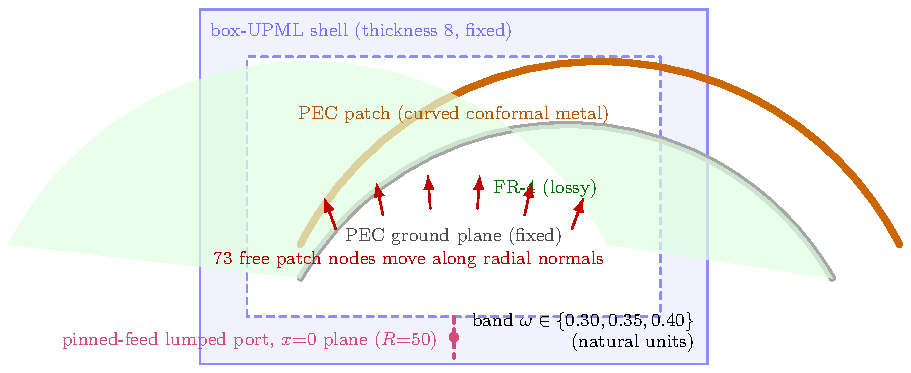
\includegraphics[width=0.72\linewidth]{figures/setup_schematic}
  \caption{Schematic of the freeform curved-metal conformal radiator: an FR-4 +
  PEC patch/ground slab wrapped around a cylinder of bend radius $40$ (natural
  units, as recorded) inside a matched box-UPML shell, driven by a pinned-feed
  lumped port on the $x=0$ plane. The free patch-conductor nodes (73 active
  DOFs) move along their radial normals; the PML shell, port plane, ground
  plane, and outer boundary are held fixed.}
  \label{fig:setup}
\end{figure}

\section{Results}
\label{sec:results}

\paragraph{Fixture.}
The reported design is the \texttt{bent\_conformal} fixture: a flat FR-4 + PEC
patch/ground slab wrapped around a cylinder of bend radius $40$ (natural units)
about the $y$-axis to produce genuinely curved conformal metal, with an $8$
(natural units) box-UPML shell and an $x=0$ port plane. The discretization has
$6173$ edges, $997$ nodes, and $4875$ tetrahedra; the design vector has $73$
active freeform boundary DOFs and a $50$ (dimensionless) port resistance.

\paragraph{Gradient correctness.}
The full band gradient matches a central finite difference of the public driven
pipeline on the curved mesh to relative error $1.17\times10^{-10}$ (analytic and
central directional derivatives both $1.751288204\times10^{-1}$, FD step
$10^{-6}$, tolerance $5\times10^{-3}$), with one factorization per band
frequency.

\paragraph{Headline design result.}
Bounded backtracking steepest descent (Armijo line search) on the 73-DOF design
vector reaches a genuine \texttt{target\_reached} terminal in $6$ accepted
steps (of a $600$-step cap --- a true target hit, not a step cap), with $0$
total backtracks. The band objective~\eqref{eq:objective} falls from
$1.897943102\times10^{-1}$ to $3.411688781\times10^{-2}$, a reduction factor of
$5.56$. The worst-of-band return loss improves from $-5.51$~dB to $-12.06$~dB,
driving the \emph{entire} design band below the $-10$~dB spec. The final
per-frequency reflection is
\begin{center}
\begin{tabular}{lccc}
\toprule
$\omega$ & $0.30$ & $0.35$ & $0.40$ \\
\midrule
$|S_{11}|$ (dB) & $-12.06$ & $-23.92$ & $-14.42$ \\
$|S_{11}|$ (mag) & $0.2494$ & $0.0637$ & $0.1900$ \\
\bottomrule
\end{tabular}
\end{center}
Figure~\ref{fig:s11band} shows the convergence trajectory and the final
per-frequency return loss against the $-10$~dB target.

\begin{figure}[t]
  \centering
  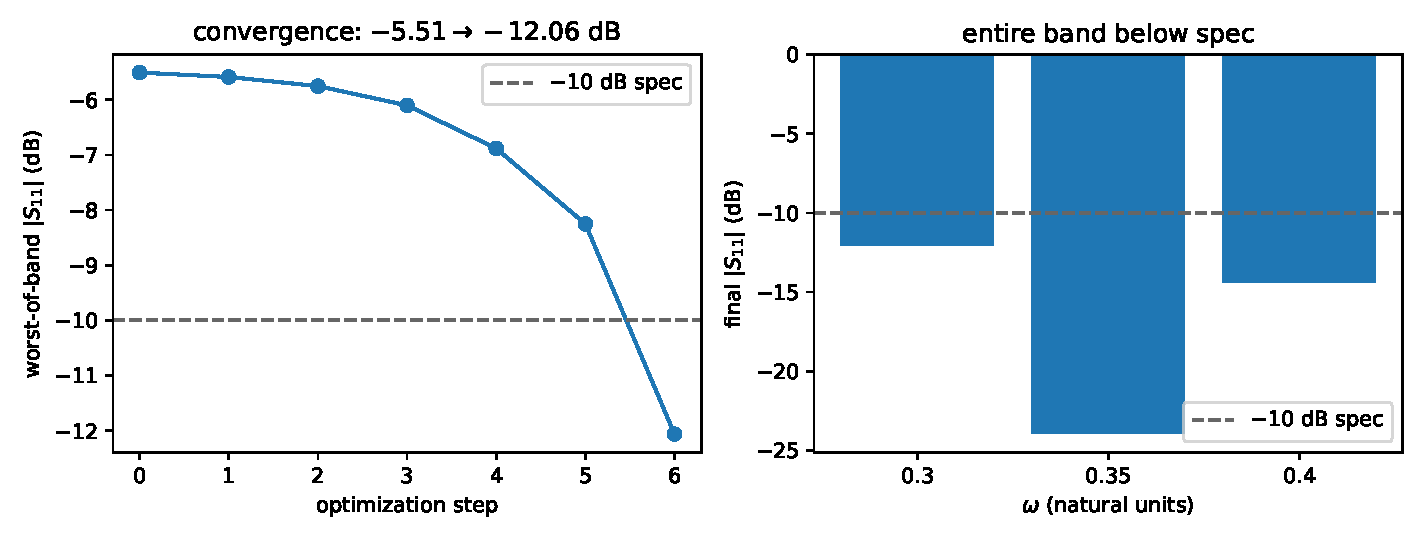
\includegraphics[width=0.9\linewidth]{figures/s11_band}
  \caption{Left: worst-of-band return loss versus optimization step
  ($-5.51 \to -12.06$~dB over $6$ accepted steps). Right: final per-frequency
  $|S_{11}|$ (dB) at $\omega\in\{0.30,0.35,0.40\}$ against the $-10$~dB spec
  (dashed). All values from the committed artifact
  \texttt{conformal\_results.toml}.}
  \label{fig:s11band}
\end{figure}

\paragraph{Guards and determinism.}
The non-inversion guard never bound: the worst per-tet signed-volume ratio was
$0.572$ against the $0.25$ budget, at a maximum nodal displacement of $0.560$
(natural units). Passivity $|S_{11}|\le 1$ held at every evaluation. The
gradient norm fell from $1.751\times10^{-1}$ to $8.987\times10^{-2}$. An
independent fresh forward band solve at the final design (public
\texttt{driven\_solve\_with\_ports}, no adjoint) reproduces the optimizer's
final band objective to relative $0.0$, and the run is bit-identical on re-run.

\paragraph{Methodological foundation.}
The composed driven SHAPE-adjoint stack --- lossy complex-$\varepsilon$ adjoint,
pinned/moving-feed lumped-port adjoint, box-UPML tensor-material adjoint --- was
validated by a prior single-DOF capstone (a separate, earlier artifact) that
retuned a flat patch through the same FD gate. The conformal result extends that
from $1$ DOF to $73$ freeform DOFs on curved geometry.

\section{Evaluation: Structured-Grid Density FDTD is Intractable on the Curved Radiator}
\label{sec:eval}

The title asserts a comparative claim --- that a structured-grid density inverse
design cannot reach this curved conformal radiator. We substantiate it not with
one head-to-head optimization but with two independent \emph{measured} axes,
both committed to the repository (Section~\ref{sec:availability}): geometric
fidelity (Section~\ref{sec:staircase}) and compute (Section~\ref{sec:runtime}).
\textbf{Honesty note.} We did \emph{not} run a converged FDTD-density
optimization of this geometry. The intractability is established by measured
scaling laws plus clearly-labelled projections; a converged FDTD-density run
would only re-confirm the intractability and is stated as future work
(Section~\ref{sec:discussion}). Every number below traces to
\texttt{benchmarks/fdtd\_density\_baseline/}.

\subsection{Geometric-fidelity axis: the staircasing error does not vanish}
\label{sec:staircase}

The \texttt{bent\_conformal} patch conductor is a circular arc (bend radius $40$;
the top and bottom conductor faces lie on radii $40.8$ and $39.2$, spanning a
$\phi_{\max}=0.3$-rad sweep, a $\sim\!24.1$-wide feature). We rasterize this arc
onto a Yee/Cartesian density grid at increasing resolution $N$ and compare its
perimeter, area, and boundary position against the exact arc
(\texttt{staircasing\_results.json}). The unstructured-tet reference is exact by
construction: its nodes lie \emph{on} the arc, so its boundary-position RMS is
$0$ to machine precision at \emph{any} resolution and at fixed DOF.

\begin{center}
\begin{tabular}{lcccc}
\toprule
$N$ & cell size & perimeter rel.\ err. & area rel.\ err. & boundary RMS \\
\midrule
$20$  & $1.206$ & $13.0\%$ & $13.58\%$ & $0.291$ \\
$40$  & $0.603$ & $15.4\%$ & $0.33\%$  & $0.157$ \\
$80$  & $0.301$ & $14.2\%$ & $0.33\%$  & $0.095$ \\
$160$ & $0.151$ & $14.2\%$ & $0.15\%$  & $0.045$ \\
\bottomrule
\end{tabular}
\end{center}

The area error converges (log-log slope $\approx\!1.96$ in $h$) and the boundary
position drifts down slowly (slope $\approx\!0.88$), but the \emph{perimeter}
error --- the quantity that sets edge-current path length and thus resonance ---
does \emph{not} converge to zero: it plateaus at a constant $\sim\!+14\%$
(log-log slope $-0.026$, i.e.\ flat) as the grid is refined. A staircased
boundary trades area accuracy for a persistent perimeter bias no amount of
uniform refinement removes. To make the rasterized boundary as faithful as the
conformal tet mesh (a $\sim\!1\,\mu$m target) requires $\sim\!6029$ cells across
the $\sim\!24.1$ feature --- $\sim\!250$ cells/mm --- which in 3-D is
$\sim\!5.35\times10^{4}$ times the Yee cells of the finest grid tested. The
conformal mesh reaches that fidelity at fixed DOF. Subpixel smoothing does not
rescue the density method on this axis: SSP~\cite{hammond2025ssp} and
SSP2~\cite{romano2026ssp2} give the Meep adjoint differentiable subpixel-accurate
binarized boundaries for the material classes it supports, but the material-grid
adjoint does not support dispersive or metallic media~\cite{meepadjointdocs},
so the curved \emph{conductor} boundary --- the quantity measured here ---
remains staircase-limited in that stack.

\subsection{Compute axis: measured $\sim\!R^3$ cells and $\sim\!R^4$ wall-clock}
\label{sec:runtime}

We measured the 3-D FDTD cost of the same box-UPML curved conformal open-radiator
problem with Meep~$1.34.0$~\cite{oskooi2010meep} (the vendored \texttt{reference/meep/docker/}
container), single-process on an AWS \texttt{m6i.4xlarge} ($16$ vCPU Intel Ice
Lake, $61$~GB RAM), timing steady-state seconds/timestep over $61$ steps after
warmup (\texttt{meep\_runtime\_scaling.json}).

\begin{center}
\begin{tabular}{lcccc}
\toprule
$R$ (cells/mm) & Yee cells & s/step & peak RAM & $\mathrm{d}t$ \\
\midrule
$4$  & $10.3$~M  & $0.233$ & $1.6$~GB  & $0.125$ \\
$6$  & $34.8$~M  & $0.742$ & $4.9$~GB  & $0.0833$ \\
$8$  & $82.6$~M  & $1.715$ & $11.3$~GB & $0.0625$ \\
$10$ & $161.3$~M & $3.386$ & $21.8$~GB & $0.05$ \\
$12$ & $278.7$~M & $5.761$ & $37.4$~GB & $0.0417$ \\
\bottomrule
\end{tabular}
\end{center}

The cells count is exactly $161280\,R^3$ (structured Yee grid); the measured
per-step time scales $\sim\!R^{2.92}$ (memory-bandwidth-bound), peak RAM
$\sim\!R^{2.89}$, and $\mathrm{d}t \propto 1/R$ (the CFL/Courant condition,
measured $0.125\!\to\!0.0417$). Because a fixed physical field-decay time then
needs $\sim\!R$ timesteps, a single forward solve scales
$\sim\!R^{2.92}\cdot R \approx R^{3.92}$, i.e.\ $\sim\!R^4$
(Figure~\ref{fig:runtime}).

\paragraph{Measured absolute anchor.}
On the same box, a single $R=8$ forward solve ran $\ge\!421$ timesteps and did
\emph{not} reach field decay within a $15$-minute window --- so
$\ge\!12$~min per forward solve and $\ge\!24$~min per adjoint gradient, at a
resolution that still badly staircases the curve ($\sim\!14\%$ perimeter error).

\paragraph{Projections (extrapolated, not measured).}
Extrapolating the measured power laws from the $R=8$ $\ge\!421$-step anchor
(these are projections, clearly \emph{not} measured runs): a $3$-frequency,
$\ge\!12$-evaluation band optimization is $\ge\!14$~hours at $R=8$ and
$\ge\!70$~hours at $R=12$ (the $\sim\!R^{3.92}$ scaling of the $R=8$ lower
bound). Peak RAM hits $\sim\!60$~GB at $R=14$ and $\sim\!83$~GB at $R=16$, so
$R\!\ge\!14$ does not fit on the $61$~GB box --- a hard RAM wall well before the
curve is resolved. The resolution that would actually represent the arc
faithfully, $\sim\!250$ cells/mm (Section~\ref{sec:staircase}), implies
$\sim\!2.5\times10^{15}$ cells --- roughly $30\times$ beyond the RAM wall before
any timestep cost is counted.

\begin{figure}[t]
  \centering
  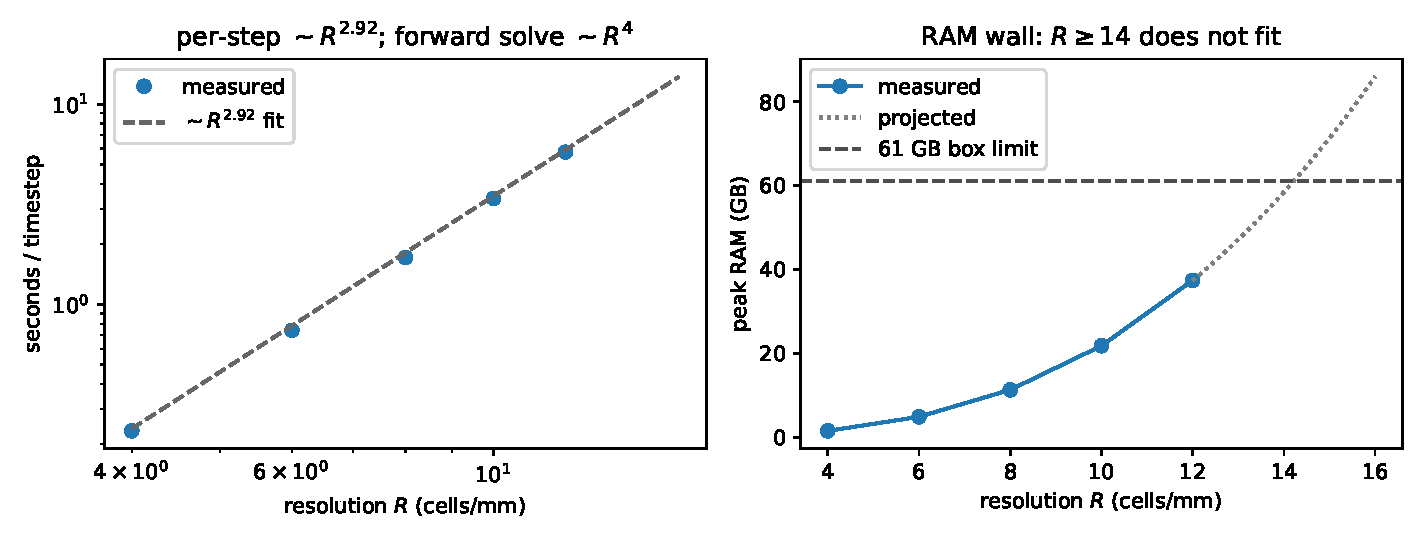
\includegraphics[width=0.9\linewidth]{figures/runtime_scaling}
  \caption{Measured Meep $1.34.0$ FDTD cost for the curved conformal
  open-radiator problem on AWS \texttt{m6i.4xlarge}. Left: seconds/timestep
  versus resolution $R$ (cells/mm), with the fitted $\sim\!R^{2.92}$ power law;
  a single forward solve adds a factor $\sim\!R$ (CFL steps), giving
  $\sim\!R^4$. Right: peak RAM versus $R$ with the $61$~GB box limit marked ---
  $R\!\ge\!14$ (projected) does not fit. Points are measured
  (\texttt{meep\_runtime\_scaling.json}); the shaded region is projected. Even
  the largest measured $R=12$ still staircases the conductor ($\sim\!14\%$
  perimeter error).}
  \label{fig:runtime}
\end{figure}

\subsection{Head-to-head}
\label{sec:headtohead}

The two axes combine into the comparative claim. On the geometric axis, a
structured Yee grid cannot represent the curved conductor without a persistent
$\sim\!14\%$ perimeter bias unless refined to $\sim\!250$ cells/mm; on the
compute axis, that resolution --- indeed any resolution past $R\!\approx\!14$ ---
is computationally intractable for single-process, single-node Meep~$1.34.0$ on
a $61$~GB host ($\sim\!R^3$ cells, $\sim\!R^4$ wall-clock, a RAM
wall on that $61$~GB box, $\sim\!10^{15}$ cells at curve-faithful resolution;
the higher-resolution and multi-node cost is a labeled projection, and
distributed or GPU FDTD would move the wall at added engineering cost). The
present unstructured-tet N\'ed\'elec shape adjoint, by contrast, solved the full
$73$-DOF freeform curved-conformal band match to worst-of-band $-12.06$~dB in
$6$ optimization steps, one reused factorization per band frequency, in
seconds-to-minutes, exact at fixed DOF with no staircasing
(Section~\ref{sec:results}). The conclusion the title asserts is therefore
measured, not merely motivational: structured-grid density FDTD is not just less
accurate on this curved open radiator --- as measured for single-process,
single-node Meep~$1.34.0$ on the $61$~GB box, it cannot practically reach the
design at the resolution the geometry demands.

\paragraph{Scope of the intractability claim.}
The compute axis is deliberately a \emph{matched} comparison --- matched
conformal-boundary fidelity, single-process, open-source density-adjoint
tooling (Meep~$1.34.0$) --- and two prior-art objections deserve naming
precisely because this scoping answers them. First, precomputed
numerical-Green-function (PNGF) inverse design~\cite{sun2025pngf} achieves
near-real-time full-wave, lumped-port-driven antenna design --- with fabricated
5G prototypes and reported speedups up to $16{,}000\times$ over commercial
solvers --- via direct binary search over a pixelated design region; so
``structured-grid antenna inverse design'' is emphatically \emph{not}
intractable in general. PNGF is fast precisely because it forgoes both adjoint
gradients and curved-boundary fidelity, so it does not reach the freeform
curved-metal design class measured here. Second, hardware-accelerated FDTD such
as Tidy3D~\cite{tidy3dautograd} would move the wall-clock and RAM walls at
added (closed-source, cloud-execution) cost --- but the geometric-fidelity axis
(Section~\ref{sec:staircase}) and the absence of metal-shape gradients
(Section~\ref{sec:related}) are unchanged by faster hardware.

\section{Discussion}
\label{sec:discussion}

The result substantiates a narrow but clean claim: a differentiable-by-construction
open-radiator FEM \emph{reaches} a freeform curved-conformal $-10$~dB design by
moving conductor-boundary nodes on a body-fitted mesh, with an exact,
single-factorization shape adjoint and enforced physics guards; and a
structured-grid density method cannot practically reach the same design at the
resolution the curved geometry demands (Section~\ref{sec:eval}). The design
space is genuinely high-dimensional (73 independent DOFs; not one parametric
knob), and the geometry is genuinely curved --- the two properties that motivate
a body-fitted node-motion adjoint over a structured density field.

\paragraph{Limitations and threats to validity.}
The scope of v1 is impedance match $+$ bandwidth only; radiation pattern and
gain (a near-to-far-field adjoint) are not addressed here. The GEODE design
result is a single fixture at one bend radius and one band; we have not swept
mesh resolution, bend radius, or band placement, so we make no claim about
generality across radiator families --- the comparative evidence in
Section~\ref{sec:eval} is what lifts this from ``one validated run'' to a
capability claim, but the reachability demonstration itself remains
single-fixture and a sweep is warranted. On the comparative side, we are careful
about what is and is not measured: the two intractability axes (staircasing,
runtime scaling) are \emph{measured}; the full-optimization wall-clock figures
($\ge\!14$~h at $R=8$, $\ge\!70$~h at $R=12$) and the RAM wall at $R\!\ge\!14$
are \emph{projections} extrapolating measured power laws from a measured
$\ge\!421$-step anchor --- we did not run a converged FDTD-density optimization.
We also note a reproducibility detail in the spirit of full disclosure: an
initial optimization run mis-recorded a premature (step-cap) stop as a physics
limit; a corrected line search reached the true \texttt{target\_reached}
terminal, which is the run reported here.

\paragraph{Future work.}
A converged FDTD-density optimization of this geometry --- which would re-confirm
the intractability rather than overturn it --- and a low-DOF parametric baseline
remain to be run. A near-to-far-field (NTFF) shape adjoint extending the
objective from $|S_{11}|$ to pattern/gain is future work and is not claimed here.

\section{Conclusion}
\label{sec:conclusion}

We presented a tensor-compiled, differentiable-by-construction 3-D N\'ed\'elec
H(curl) FEM that exposes an exact, single-factorization discrete shape adjoint
through the full open-radiator forward --- matched box-UPML tensor material,
lumped ports, lossy complex-$\varepsilon$, and a passive $|S_{11}|$ --- on
unstructured tetrahedral meshes. Driving a 73-DOF harmonic freeform boundary
morph, we gradient-designed a curved-metal conformal radiator that drives the
entire design band below $-10$~dB return loss (the per-frequency and
worst-of-band figures are reported in full in Section~\ref{sec:results}), with
the band gradient FD-validated to relative error
$1.17\times10^{-10}$, enforced passivity, and a non-inversion guard. We then
\emph{measured}, on two committed axes, that a structured-grid density method
cannot practically reach the same design: the staircasing perimeter error
plateaus at $\sim\!+14\%$, and the FDTD cost scales as $\sim\!R^3$ cells and
$\sim\!R^4$ wall-clock, hitting a RAM wall (measured for single-process,
single-node Meep~$1.34.0$ on a $61$~GB host; higher-resolution and multi-node
cost stated as a labeled projection) well before the curve is resolved.
The contribution is the narrow, previously-unoccupied combination of
Section~\ref{sec:whitespace} --- explicitly not a first EM shape adjoint. A
converged FDTD-density optimization and a pattern/gain NTFF adjoint are the
announced next steps.

\section*{Artifact and code availability}
\label{sec:availability}
All quantitative claims trace to artifacts committed on the \texttt{main} branch
of the GEODE-FEM repository, publicly available at
\url{https://github.com/rjwalters/geode-fem}. The headline design result is
\texttt{benchmarks/patch\_antenna\_conformal/conformal\_results.toml}. The
evaluation-section measurements are in \texttt{benchmarks/fdtd\_density\_baseline/}:
the geometric-fidelity axis in \texttt{staircasing\_results.json} and the compute
axis in \texttt{meep\_runtime\_scaling.json} (with \texttt{RUNTIME\_SCALING.md}).
The FDTD-density baseline itself is the vendored Meep $1.34.0$ container under
\texttt{reference/meep/docker/} (\texttt{conformal\_baseline\_3d.py}). The
shape-adjoint implementation lives in
\texttt{crates/geode-core/src/driven/shape.rs},
\texttt{crates/geode-core/src/shape.rs},
\texttt{crates/geode-core/src/mesh/patch.rs}, and the runnable example
\texttt{crates/geode-core/examples/patch\_conformal\_diffopt.rs}.

\bibliographystyle{plainnat}
\bibliography{refs}

\end{document}
